\documentclass[14pts]{report}
\usepackage{fancyhdr}
\usepackage{graphicx}
\usepackage{url}
\usepackage{natbib}
\usepackage{amsmath}
\usepackage{babel,blindtext}


\usepackage{tikz,pgfplots,pgf}
\usetikzlibrary{matrix,shapes,arrows,positioning}

\fancyhead{}
\fancyhead[LO, LE]{\rightmark}

\title{
	\begin{center}
	{Convolutional Neural Network-based medical checkup system for Pigmented Skin Lesions Classification.} \\
	\vspace{5mm} %5mm vertical space
	
	\large {
		{School of Computing, Engineering and Mathematics}\\
		{Coventry University}\\
	}
	\vspace{3mm} %3mm vertical space
	\textbf{ Bsc Computer Science}\\
	{\large Project Supervisor: Dr.David Croft}\\
	{\large Submission Date: 21/04/2020} \\
	\end{center}
}
\author{
	{\large Author Name:  Vinayak Sareen} \\
	{\large Student Id Number:  7651331} \\
	{\large Ethics Application Number: P101878 }\\
}
\date{}
\pagestyle{fancy}
\begin{document}
\maketitle

\chapter*{Statement of originality}
\subsection*{Declaration of originality}
I Declare that This project is all my own work and has not been copied in part or in whole from any other source except where duly acknowledged.  As such, all use of previously published work (from books, journals, magazines, internet etc.) has been acknowledged by citation within the main report to an item in the References or Bibliography lists. I also agree that an electronic copy of this project may be stored and used for the purposes of plagiarism prevention and detection.
\subsection*{Statement of copyright}
I acknowledge that the copyright of this project report and any product developed as part of the project, belong to Coventry University. 
Support, including funding, is available to commercialise products and services developed by staff and students. 
 Any revenue that is generated is split with the inventor/s of the product or service. 
For further information please see www.coventry.ac.uk/ipr or contact ipr@coventry.ac.uk.
\subsection*{Statement of ethical engagement}

I declare that a proposal for this project has been submitted to the Coventry University ethics monitoring website (https://ethics.coventry.ac.uk/) and that the application number is P101878.
\subsection*{}
Sign: \textbf{Vinayak Sareen}. \hspace{20mm}  Date:  \textbf{07/03/20}



\chapter*{Abstract}
Abstract should be a succinct and self-standing summary of the basis, context and achievements of the project. Minimally an abstract does three things: (1) It states the problem that you set out to solve, (2) It describes your solution and method, (3) It states a conclusion about the success of the solution. Be straightforward and factual and avoid vague statements, confusing details and "hype". Do not be tempted to use acronyms or jargon to keep within the half-page limit. Consider that search engines, librarians and non-computer scientists wishing to classify your Report rely on the abstract. You may if you wish provide a short list of keywords (2-6 is reasonable) at the end of the abstract.

\tableofcontents

\chapter*{Acknowledgements}
I want to express my gratitude to my supervisor Dr David Croft for guiding me thought the investigations. The support of all medical professionals who contribute by providing data to the research is sincerely acknowledged. At last, I would thank my parents, who supported me finically and psychologically throught this journey of computer science.

\chapter{Introduction}
\section{Introduction}
\paragraph*{}

Skin cancer is categorized into two types: melanoma skin cancer. 
Detection and classification of unknown pigmented skin lesions can result in early diagnosis of the medical problem. Melanoma is the most dangerous kind of skin cancer accounted for an estimated 16,000 deaths each year from 2014 to 2016 in the United Kingdom (Cancer Research UK, 2020). The melanoma tumour caused by melanocytes can result in uncontrolled and abnormal growth which can spread in the human body (Korotkov and Garcia 2012).
The previous research in 2017 has shown that melanoma was the 20th most common disorder with new incidents of 81,00 and 83,00 in males and females in the United Kingdom \citep*{KOROTKOV201269}.
Dermoscopy is a non-invasive method of examining the pigmented skin, which includes microscopic imaging of the surface structure of pigmented skin lesions \citep*{KOROTKOV201269}.
Early diagnosis of pigmented skin lesions is crucial to classify skin disorders to decrease mortality concerning particular skin disorders. Dermoscopy improves the detection of melanoma compared to detection of disease with naked eyes by analysing the pigmented skin lesion. Previous studies have shown that such tumours can result in higher chances of better treatment and cure of disease by removing the tumour \citep*{CELEBI2007362}.
The current diagnosis method of detection involves using ABCD rule which considers the Asymmetry, Border irregularity, Colour irregularities, Darmascopic structures respectively of common pigmented skin lesions \citep*{LOESCHER2013170}.
People working in busy work environments or less mobility can be victims of belated and slow diagnosis of such dangerous skin cancers.
The automated analysis of pigmented skin lesions using artificial neural networks can be beneficial in optical analysis of microscopic images of pigmented skin lesions. 
The primary targeted audience who benefits from the outcome is the people who are working in busy work environments or people with less mobility are best to use cases which can use such an automated system. Booking a prior appointment with medical professionals based on the urgency of detected medical problems can result in the immediate treatment of patients with more critical conditions. The people with less mobility such as older audiences or people with special needs can detect pigmented skin lesions through online systems in an inconvenient manner. Medical institutions can use such technologies to automate the process of pre-health checkups and overcome the problem of shortage of staff members in case of emergency. Such automated systems can also result in faster diagnosis of medical problems compared to a manual analysis by a clinician. 
Furthermore, manufacturing companies which supply the microscopic medical instruments can also use such intelligent models with their products to provide value to customers and medical institutions.

\paragraph{ The research concentrates}
on developing a type of artificial neural network called a convolutional network to perform automated optimal analysis to identify the class of pigmented skin lesion. 
The research focuses on providing the quantitative analysis on comparing the results predicted by the automated intelligent machine are compared with medical professionals to identify the classes of pigmented skin lesions. The study employs different experiments by applying different model architectures and analysing accurate hyper-parameters for optimal performance. 
The research concentrate on analysing disorders such as melanoma, benign keratosis, melanocytic nevi and basal cell carcinoma. The investigation employs publicly available HAM10,000 dataset. 
The extensive collection of 10,000 images of labelled data units were collected from a diverse population of subjects over twenty years.


\section{Pigmented Skin Lesions}
1. Melanoma. 
2. Benign keratosis-like lesions.
3. Melanocytic nevi. 
4. Vascular lesions.
\pagebreak
\pagebreak
\section{Bioligical Inspiration for Neural Networks}
The human brain are componsed of millions specialised cell "neurons" which are interconnected to each other which carry electrical and chemical signals from neuron to another to function
There are an estimated 500 trillion connections between neurons in the human nervous system which helps communicate signals \citep*{patterson2017deep}.
The fundamental component of neural networks, which is the perceptron model, is inspired by the single neuron structure.
\subsection{Structure of Neurons}
\vspace{3mm}
\begin{center}
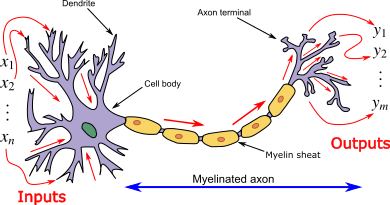
\includegraphics[width=10cm]{Images/neuron.png}
\end{center}

The figure above represents the biological structure of neurons that helps in the communication of electric signals in the nervous system to learn and process information. The biological structure of neurons
includes three major parts dendrites which are responsible for accepting the electrical and chemical signals to the neuron. 
Furthermore, the neuron contains the nucleus which is accountable for the processing input information with the neurons. 
At last, the processed information is passed to another neuron which is interconnected to neurons in the human nervous system through axon terminals
\citep{AGATONOVICKUSTRIN2000717}. 

\subsection{Perceptron Model}
\pagebreak
\section{Artifical Neural Networks}
In this section, you should describe the problem that you set out to solve with the project. An introduction might, for example, begin by stating, "The aim of the work described in this Report was to provide a software tool with which people can arrange meetings." Avoid starting a Report with an irrelevant history of information technology. For example, the following would not be a good introductory sentence, "Since Bill Gates launched Outlook people have been using technology to arrange meetings."
Explain whatever background the reader will need in order to understand the problem. The background might refer to previous work in the academic literature that provides evidence that the problem is a real and significant problem worth solving. The background may identify a community, organisation or set of users that will benefit from your research. Include a clear and detailed statement of the project aims and provide an overview of the structure of the solution.
Explain whatever background the reader will need in order to understand the problem. The background might refer to previous work in the academic literature that provides evidence that the problem is a real and significant problem worth solving. The background may identify a community, organisation or set of users that will benefit from your research. Include a clear and detailed statement of the project aims and provide an overview of the structure of the solution.
CRITICAL! Use the introduction to define any terms or jargon that you will be using throughout the rest of the report.  Why?  Because people define and understand terms differently from one another.  Your definition of ‘cloud computing’ may be different to your supervisor’s definition of ‘cloud computing’.  By stating your definition clearly you can avoid misunderstandings of your work.
Conventionally, the last part of the introduction outlines the remainder of the Report, explaining what comes in each section – keep this brief.
In this section, you should describe the problem that you set out to solve with the project. An introduction might, for example, begin by stating, "The aim of the work described in this Report was to provide a software tool with which people can arrange meetings." Avoid starting a Report with an irrelevant history of information technology. For example, the following would not be a good introductory sentence, "Since Bill Gates launched Outlook people have been using technology to arrange meetings."
Explain whatever background the reader will need in order to understand the problem. The background might refer to previous work in the academic literature that provides evidence that the problem is a real and significant problem worth solving. The background may identify a community, organisation or set of users that will benefit from your research. Include a clear and detailed statement of the project aims and provide an overview of the structure of the solution.
Explain whatever background the reader will need in order to understand the problem. The background might refer to previous work in the academic literature that provides evidence that the problem is a real and significant problem worth solving. The background may identify a community, organisation or set of users that will benefit from your research. Include a clear and detailed statement of the project aims and provide an overview of the structure of the solution.
CRITICAL! Use the introduction to define any terms or jargon that you will be using throughout the rest of the report.  Why?  Because people define and understand terms differently from one another.  Your definition of ‘cloud computing’ may be different to your supervisor’s definition of ‘cloud computing’.  By stating your definition clearly you can avoid misunderstandings of your work.
Conventionally, the last part of the introduction outlines the remainder of the Report, explaining what comes in each section – keep this brief.
\subsection{Deep Neural Networks}


\subsection{Backpropagation}


\chapter{Literature Review}
\subsection{Convential Diagnosis Methods}

The most common conventional diagnosis method of detection involves
using ABCD rule which considers the Asymmetry, Border irregularity, Colour
irregularities,  Darmascopic structures respectively of common pigmented skin
Lesions \citep*{LOESCHER2013170}. The above method of analysis is performed on 
dermoscopic images of pigmented skin lesions.  Dermatoscopy is 
non-invasive microscopic imaging of pigmented skin lesions which provides clear imaging to perform 
proper analysis on pigmented skin lesions \citep*{LOESCHER2013170}. 
Furthermore, the result of dermatoscopic images is examined 
by dermatologists to classify the pigmented skin lesion.  \textbf{SOME SAYS ....}

\subsection{Support Vector Based Machine}
Thompson Felsia and Jeyakumar proposed research in 2017 on 
support vector machine based classifier to detect multi-lesions skin cancer by analysing pigmented skin lesions with an accuracy of 86.37 percent.
The proposed investigation with SVM based classifier has performed image segmentation using SRM (support region merging) algorithm. Furthermore, it employs SURF (speed up robust features) to find the region 
of interest for feature extraction to get optimal classification performance based on vector-based technique \citep*{thompson2017vector}. 
However, the research does not include image augmentation which generalises the predictions accurate to test in 
real-world environment. The research papers mention that support vector machine for automated classification of pigmented skin lesions is sensitive to the artefacts and can 
potentially increase the false positives which mean that predicted result for analysis was wrong positive prediction instead of an actual negative result. The investigation will perform image augmentation to generate random 
samples of images with different rotation angle and flipped images will be used to train and test the model to generalise the overall performance.

\subsection{Border Detection Based System}
Rahil Garnavi and his other co-researchers purposed research based on a state of the art border detection method combined with the colour space analysis and clustering-based histogram hybrid thresholding to classify pigmented skin lesions.
 The research was primarily focused on the research was to develop the hair removal mechanism to perform colour channels transformation. Furthermore, for all the image channels the noise reduction 
and clustering-based histogram thresholding were performed for optimal border detection. The predicted outcomes of novel broder detection system were compared with the 
borders detected by the actual dermatologists on a sample of 
dermoscopic pigmented skin lesions to understand the reliability of the 
system \citep*{GARNAVI2011105}.However, the system was only tested on a data sample set of 
30 dermoscopic images and four sample sets of dermatologist hand-drawn images were used as ground truth to compare the results. The system was tested on overall 85 dermoscopic images.
Border detection can be used to analyse the pigmented skin lesions but convolutional networks have the potential to find more data patterns in the images to minimise the cost function 
using the backpropagation algorithm. The current research will 
employe basic image segmentation based on the binary threshold 
algorithm as an experiment to help network detecting more accurate
borders of pigmented skin lesions.

\subsection*{Deep Feature to classify Pigmented Skin lesions}

In 2016, a research paper from Simon Fraser University’s computer science and medical image analysis lab had researched using 
deep residual network architecture with ten labelled 
classes of pigmented skin lesions. The research was based on very 
deep convolutional network architecture with the accuracy 
of 85.8 percent in classifying five distinct classes and
81 percent in classifying 10 classes of pigmented skin lesions
\citep*{7493528}. Although the performance of the overall convolutional network was accurate, the training and testing data were limited to 13,00 overall images of 10 distinct classes.
 However, In the current research project, the classes of labelled images will be five and around 9,000 overall images will be used during the investigation.
 Estimated 80 percent of data will be consumed for training the model, and the rest of the label images will be used as validation and testing datasets 
 to evaluate the performance of the model. 
 Research is also consuming such artificial neural network-based technologies to various areas of investigations.

\chapter{Methodology}
The research purposes a solution based on deep convolutional neural networks with various experiments mentioned in further sections.
The operations require machine learning specific configuration for Cuda libraries and configuration to run programs on available GPU(Graphical Processing Unit) for faster processing and further, 
instructions to setup environment can be found at \url{https://www.tensorflow.org/install/gpu}. In addition, convolutional neural network was implmented using Python3 and jupyter notebooks were used in these experiments 
which provides an appropriate interface to experiment and write markdowns.
The data science and machine learning libraries such as NumPy for numerical operations, matplotlib for visualisation, Keras for developing deep learning models and OpenCV for image processing was used in the process of developing an automated system for classifying pigmented skin lesions.
HAM,1000 dataset was used to train image classifier, which can be found at
\url{https://dataverse.harvard.edu/dataset.xhtml?persistentId=doi:10.7910/DVN/DBW86T}. The dataset contains two folders containing dermatoscopic images of pigmented skin lesion and CSV file which contains meta information and image name for each pigmented skin lesion.

\section{Data Processing and Normalisation}
Datasets contain unclear and hairy images of pigmented skin lesions which were manually 
removed from the dataset to enhance the quality of available data. The information was read using pandas into the data frame, 
which is a data structure that allows storing tabular data from CSV files. The CSV file contained irrelevant information such as gender and age of 
patients and unbalanced data classes data columns were dropped from the dataset. Furthermore, the dataset was divided into training and 
testing sets using \url{sklearn.model_selection.train_test_split} class in the portion of 80 per cent for 
the training dataset and 20 per cent of testing datasets. The next step towards to preparing the dataset was reading the images data into NumPy 
array for both training and testing datasets and converting the image names from pandas series to NumPy array corresponding to each image and assign class number 
based on category of pigmented skin lesion in the dataset. Furthermore, the training and testing datasets were serialised into 
dictionary in a pickle encoded file. Therefore, the encoded file sizes are compact and are portable
in comparison to storing actual image files.

\subsection{Data Normalisation}
The images RGB images numpy array was mutli-demensional array with numbers ranging from 0 to 255.
The numpy array was converted into the float32 format and each element of the array was divided by 255 to normalise the data so, that 
it only ranges between 0 and 1 in float format which will help while training the model. In addition, one hot encoding 
was performed on class labels of the pigmented lesions. The one hot encoding is a representation of categorical variable 
as binary vector and normalise the categorical labels into binary vector.

\subsection{ Image Segmentation }
\begin{center}
	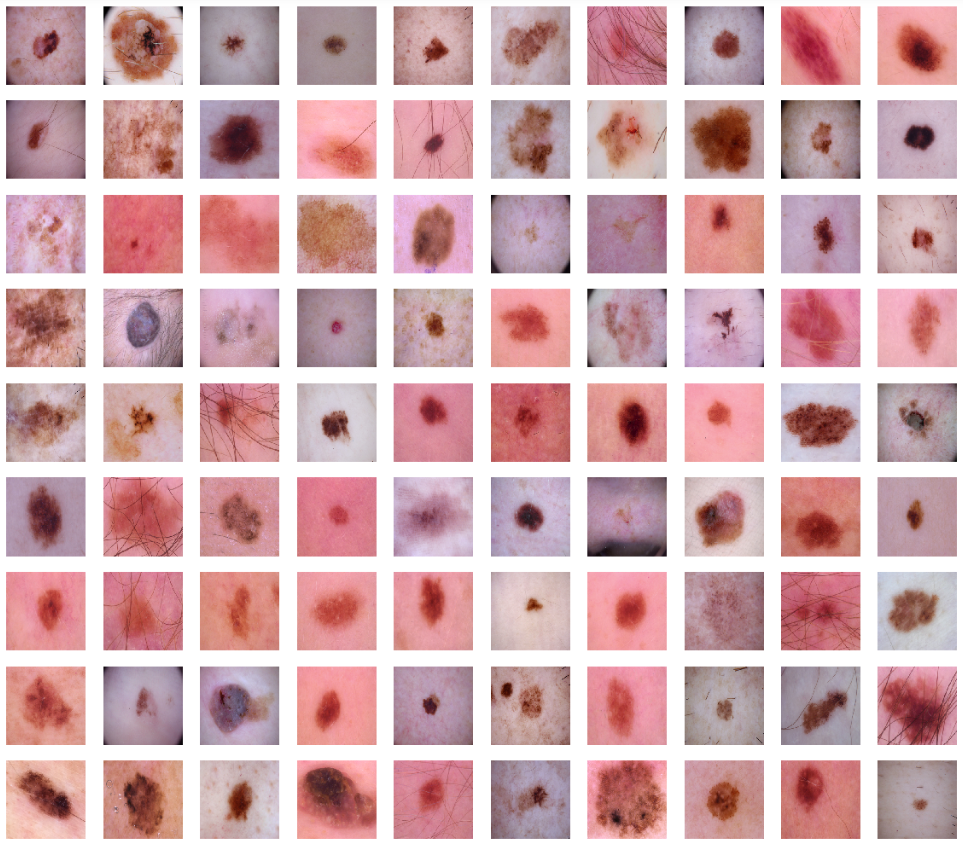
\includegraphics[width=10cm]{Images/bseg.png}
\end{center}

The figure above reflects the sample from training dataset before performing image segmentation.
The image segmentation was performed on the all the images using binary thresholding in OpenCV framework.

\section{Thresholding Segmentation Algorithm}

Thresholding is one of the commonly adopted method in image segmentation which helps in descrimination most 
significant pixels in the images \citep*{al2010image}. The thresold value is selected and the gray scale images  
are converted into the binary representation of the image and value of image which are greater than the thresold
value will be selected with keeping all the attributes of the images such as position and shape \citep*{al2010image}. 
Thus, reducing the complexity of the image data and making it easier for classification related tasks. Futhermore, the 
segmented images will be consumed in the model training. The thresholding segmentation was performed using OpenCV library using 
\url{cv.threshold(image, 0.5, 1, cv.THRESH_BINARY)} where threshold value of 0.5 and maximum value of the pixel can be 1
as it was normalised.

\begin{center}
	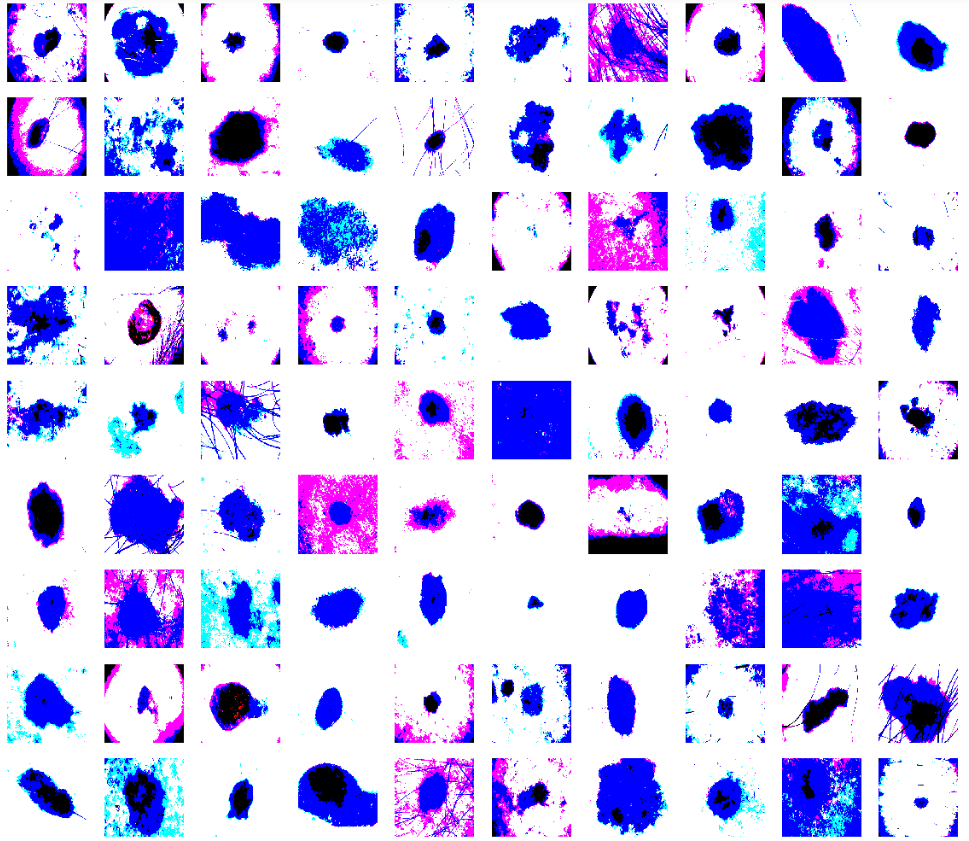
\includegraphics[width=10cm]{Images/aseg.png}
\end{center}

The figure above shows the result of applying the threshold image segmentation on pigmented skin lesions. 




\chapter{Evaluations and Results}
In this chapter, you should evaluate what you have done, and say what answer (to your research question) you have arrived at. It may be that in your method you describe some experiments, and this section records your results and analysis of those results. This is an important section -- most students gain or lose marks in either their literature review or evaluation. The key to producing a convincing evaluation is to plan very early in the project what information or results you will need to write this section.

\chapter{Project Managment}
\subsection*{Meeting Logs with Supervisor}
\subsection*{Software Development Lifecycle}
\subsection*{Work Managment System}
\begin{figure}[!htp]
    \centering
    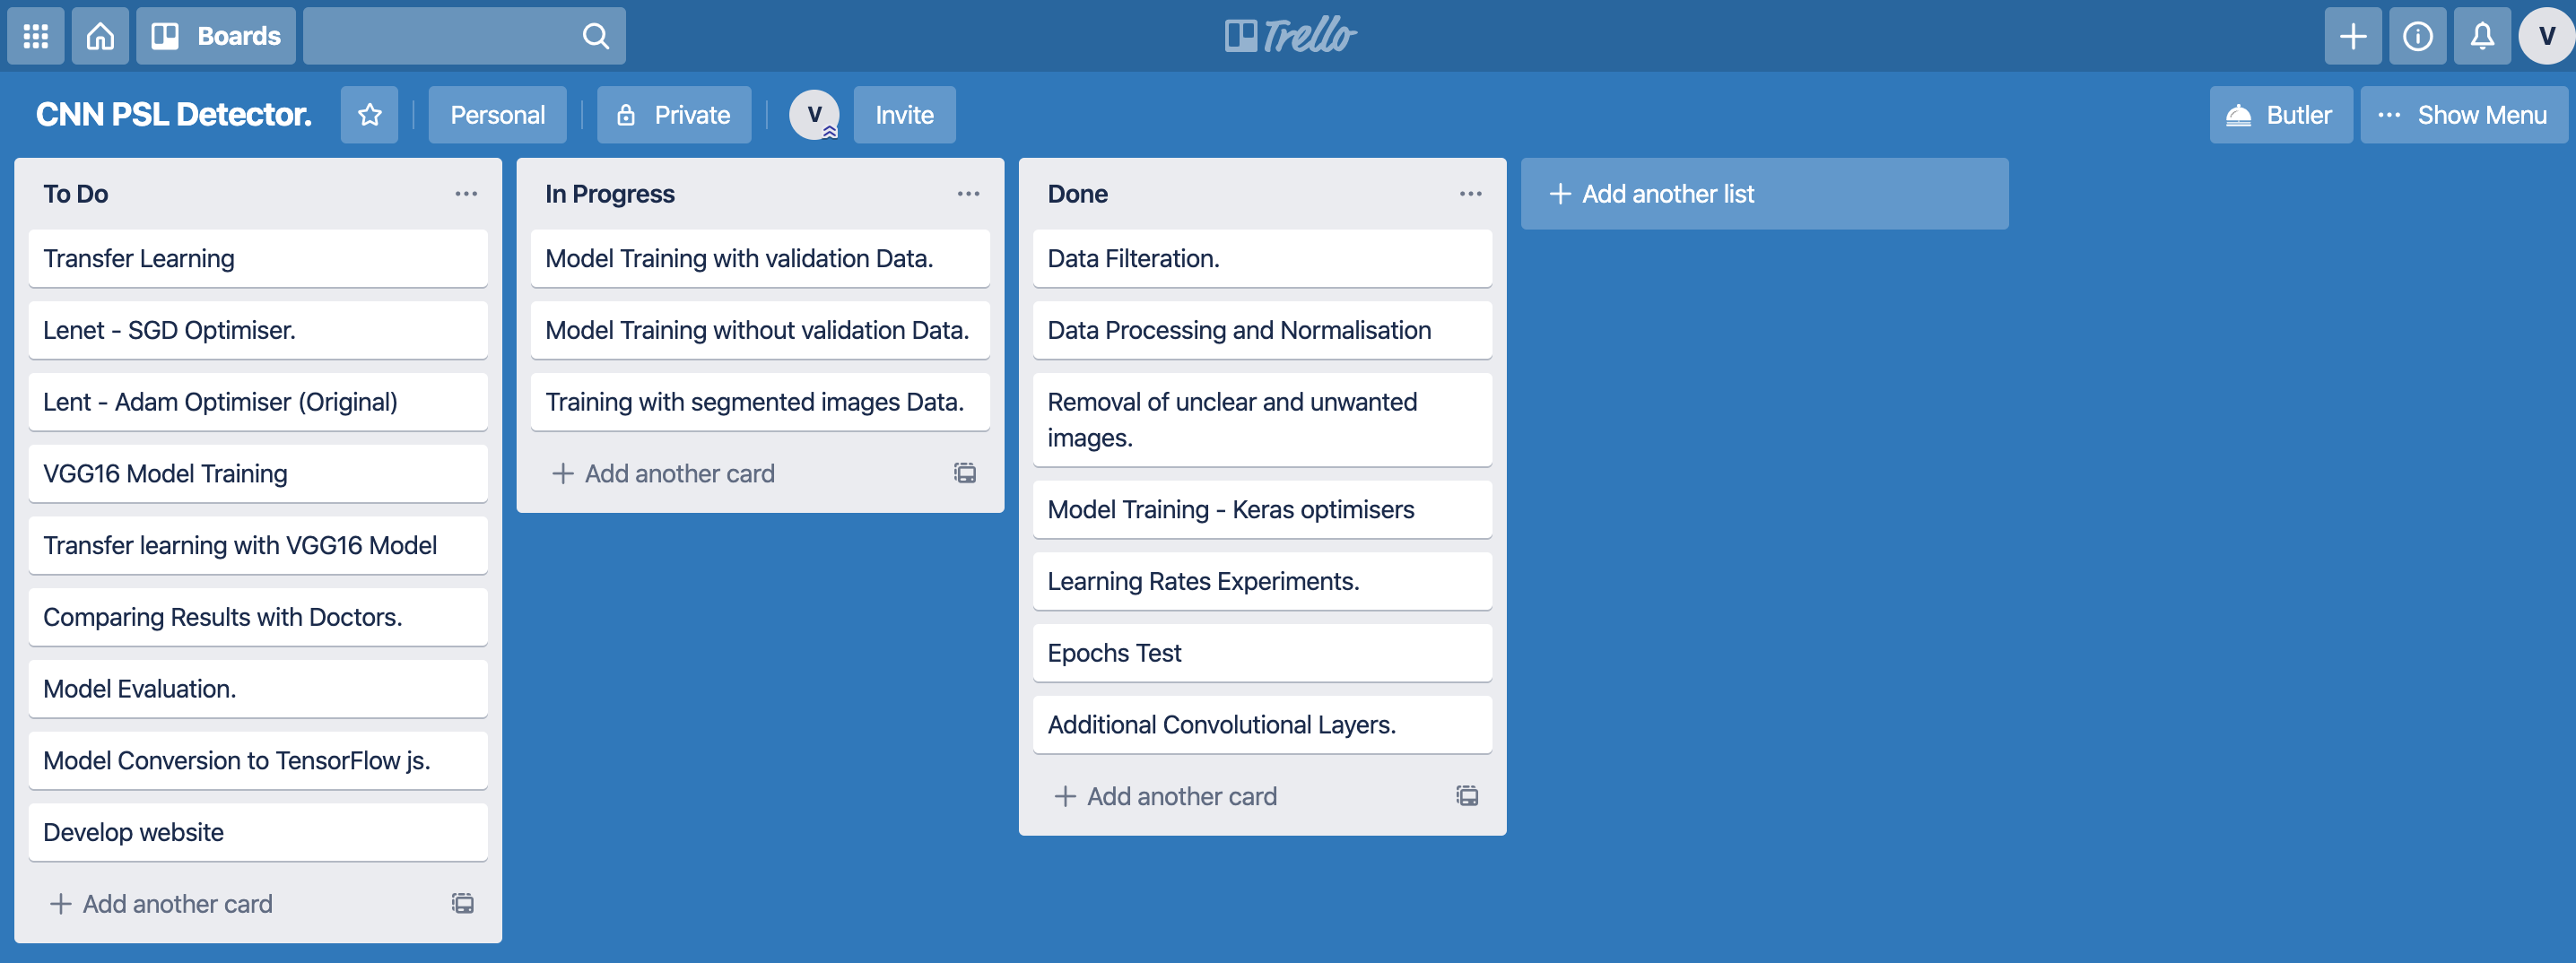
\includegraphics[width=15cm]{Images/Kanban Bords.png}
    \caption{Kanban Board}
\end{figure}
\subsection*{Version Control}





\chapter{Reflection}
This is dummy text for reflection

\chapter{Conclusion}
CONCLUSION is pending

\bibliographystyle{agsm}
\bibliography{./References}

\chapter{Appendices}
\section*{Participation Consent Form}
\begin{center}
    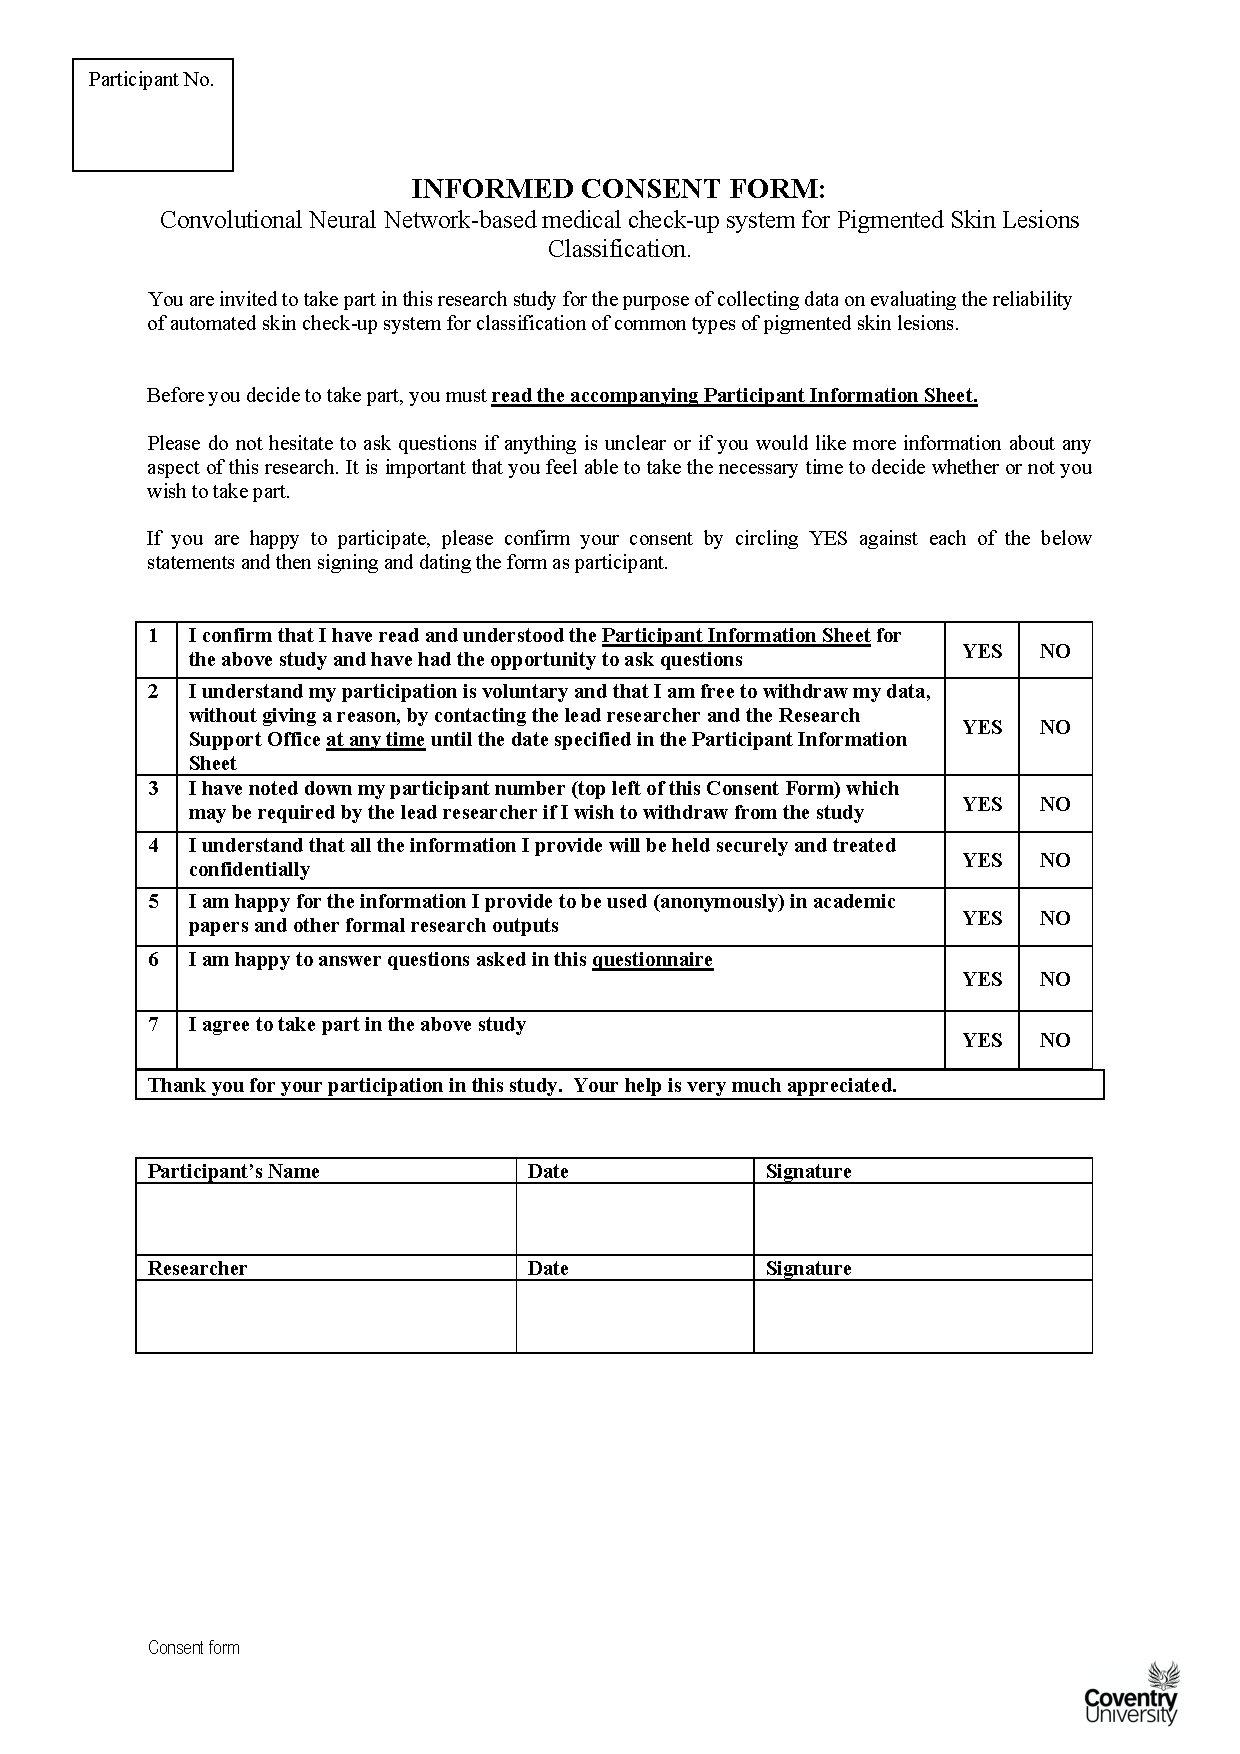
\includegraphics[width=15cm]{Documents/consent.pdf}
\end{center}

\section*{Participation Information Sheet}
\begin{center}
    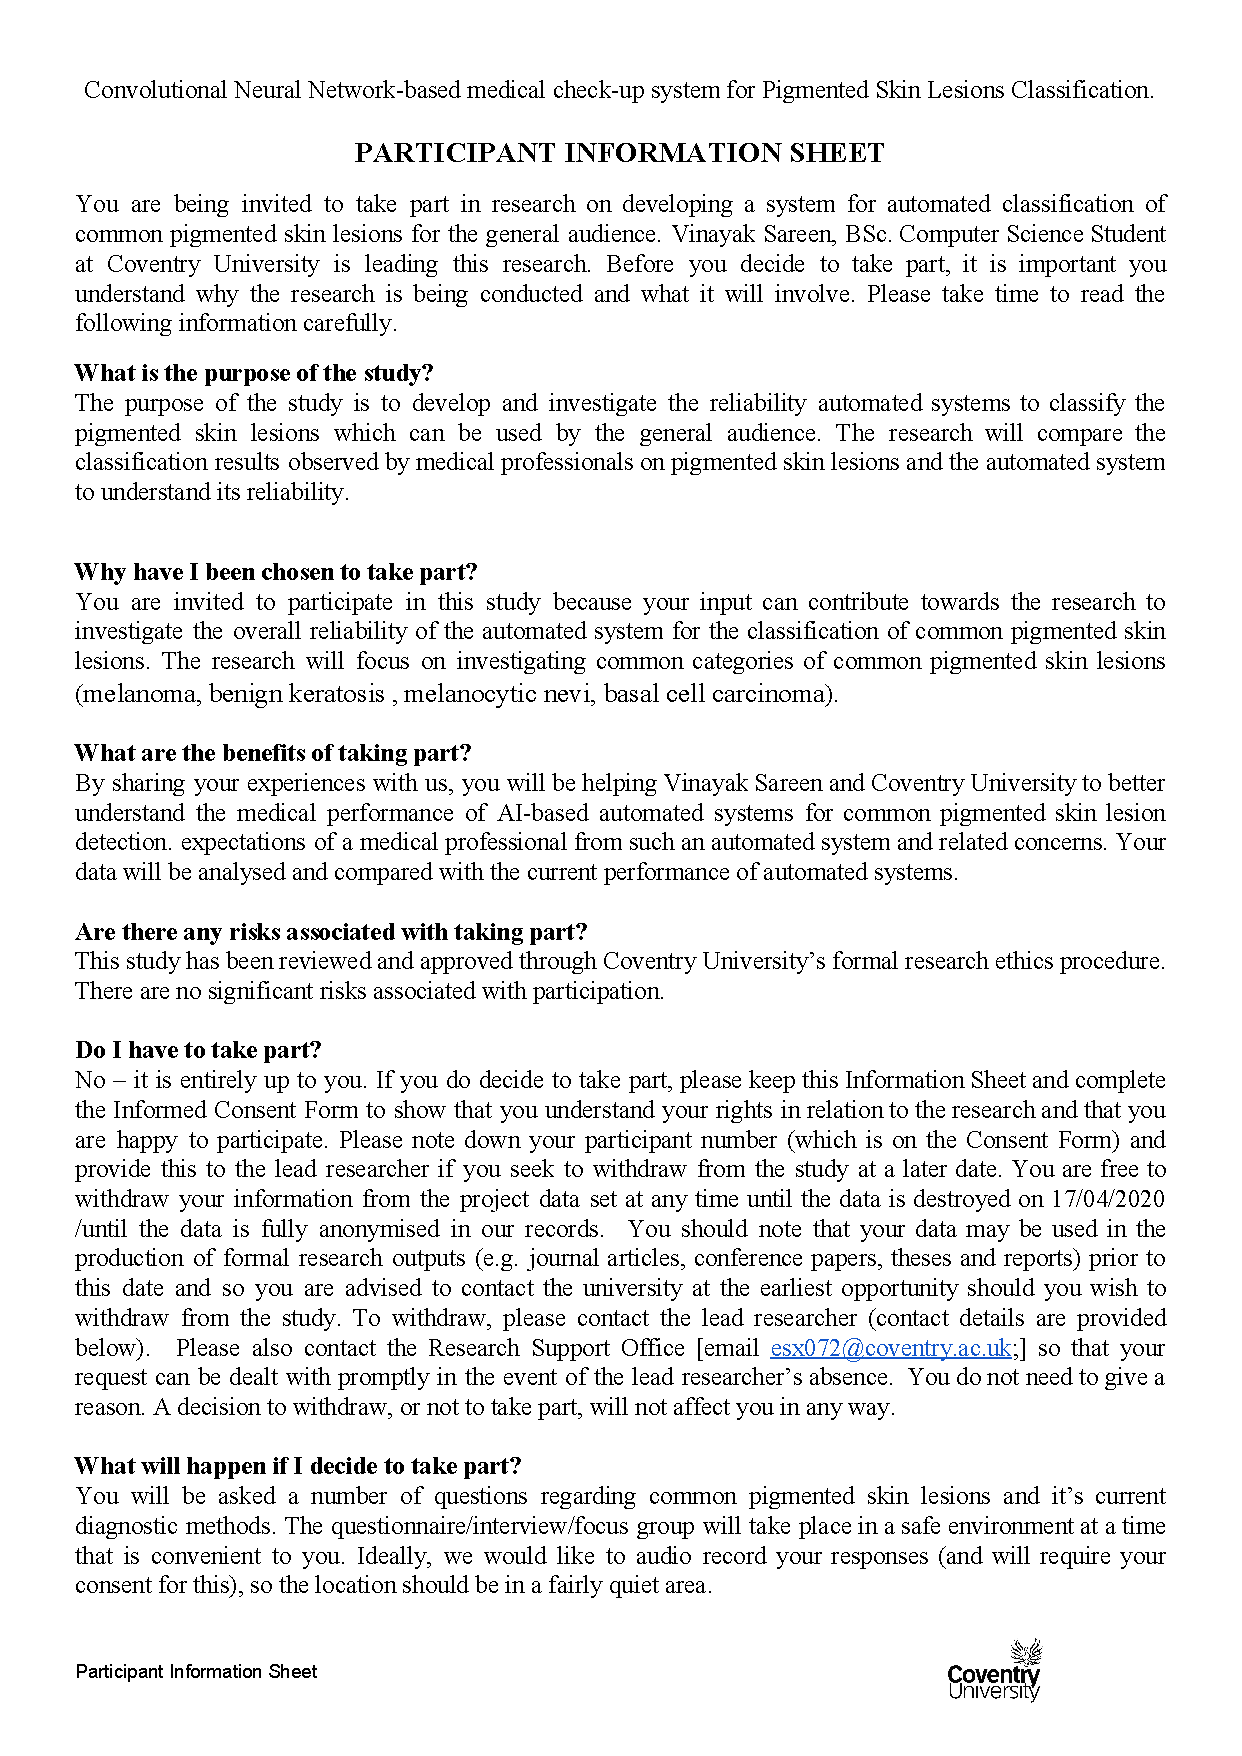
\includegraphics[width=15cm]{Documents/participation.pdf}
\end{center}

\section*{Supervisor Meeting Logs}
\addcontentsline{toc}{chapter}{Appendices}
\end{document}